% ============================================================
% Question Bank: ch04-07 Laws of Exponents
% Topic Title: Laws of Exponents
% CCSS: Supplementary / 8.EE.A.1 (Preview)
% Questions: 27 (15 MC + 6 SA + 6 Graphical)
% ============================================================

% --- Multiple Choice Questions (15) ---

\begin{practiceQuestion}{4-7-q01}{mc}
\begin{questionText}
Simplify $5^3 \times 5^4$.
\end{questionText}
\choiceA{$5^{12}$}
\choiceB{$25^7$}
\choiceC{$5^7$}
\choiceD{$5^{7} \times 2$}
\correctAnswer{C}
\explanation{Product rule: $5^3 \times 5^4 = 5^{3+4} = 5^7$.}
\end{practiceQuestion}

\begin{practiceQuestion}{4-7-q02}{mc}
\begin{questionText}
Simplify $\dfrac{8^9}{8^5}$.
\end{questionText}
\choiceA{$8^{45}$}
\choiceB{$8^4$}
\choiceC{$1^4$}
\choiceD{$8^{14}$}
\correctAnswer{B}
\explanation{Quotient rule: $\frac{8^9}{8^5} = 8^{9-5} = 8^4$.}
\end{practiceQuestion}

\begin{practiceQuestion}{4-7-q03}{mc}
\begin{questionText}
Simplify $(4^2)^3$.
\end{questionText}
\choiceA{$4^5$}
\choiceB{$4^8$}
\choiceC{$4^6$}
\choiceD{$4^{23}$}
\correctAnswer{C}
\explanation{Power of a power rule: $(4^2)^3 = 4^{2 \times 3} = 4^6$.}
\end{practiceQuestion}

\begin{practiceQuestion}{4-7-q04}{mc}
\begin{questionText}
What is the value of $7^0$?
\end{questionText}
\choiceA{$0$}
\choiceB{$7$}
\choiceC{$1$}
\choiceD{$70$}
\correctAnswer{C}
\explanation{Any nonzero number raised to the zero power equals $1$. So $7^0 = 1$.}
\end{practiceQuestion}

\begin{practiceQuestion}{4-7-q05}{mc}
\begin{questionText}
Which expression is equivalent to $2^5 \times 2^3$?
\end{questionText}
\choiceA{$4^8$}
\choiceB{$2^{15}$}
\choiceC{$2^8$}
\choiceD{$4^{15}$}
\correctAnswer{C}
\explanation{Product rule: $2^5 \times 2^3 = 2^{5+3} = 2^8$.}
\end{practiceQuestion}

\begin{practiceQuestion}{4-7-q06}{mc}
\begin{questionText}
Simplify $\dfrac{6^{10}}{6^{10}}$.
\end{questionText}
\choiceA{$6^{100}$}
\choiceB{$0$}
\choiceC{$6^0 = 1$}
\choiceD{$6^{20}$}
\correctAnswer{C}
\explanation{Quotient rule: $\frac{6^{10}}{6^{10}} = 6^{10-10} = 6^0 = 1$.}
\end{practiceQuestion}

\begin{practiceQuestion}{4-7-q07}{mc}
\begin{questionText}
Which exponent law justifies $a^m \times a^n = a^{m+n}$?
\end{questionText}
\choiceA{Quotient rule}
\choiceB{Power of a power rule}
\choiceC{Product rule}
\choiceD{Zero exponent rule}
\correctAnswer{C}
\explanation{The product rule states that when multiplying powers with the same base, you add the exponents.}
\end{practiceQuestion}

\begin{practiceQuestion}{4-7-q08}{mc}
\begin{questionText}
Simplify $(3^4)^2$.
\end{questionText}
\choiceA{$3^6$}
\choiceB{$3^8$}
\choiceC{$9^8$}
\choiceD{$3^{16}$}
\correctAnswer{B}
\explanation{Power of a power: $(3^4)^2 = 3^{4 \times 2} = 3^8$.}
\end{practiceQuestion}

\begin{practiceQuestion}{4-7-q09}{mc}
\begin{questionText}
A student writes $\dfrac{10^6}{10^2} = 10^3$. Is this correct?
\end{questionText}
\choiceA{Yes, because $6 \div 2 = 3$}
\choiceB{No, the answer should be $10^4$ because $6 - 2 = 4$}
\choiceC{No, the answer should be $10^{12}$}
\choiceD{Yes, because you divide the exponents}
\correctAnswer{B}
\explanation{Quotient rule: subtract exponents, not divide. $\frac{10^6}{10^2} = 10^{6-2} = 10^4$.}
\end{practiceQuestion}

\begin{practiceQuestion}{4-7-q10}{mc}
\begin{questionText}
Simplify $9^2 \times 9^0$.
\end{questionText}
\choiceA{$9^2$}
\choiceB{$9^0$}
\choiceC{$0$}
\choiceD{$81^2$}
\correctAnswer{A}
\explanation{$9^0 = 1$, so $9^2 \times 9^0 = 9^2 \times 1 = 9^2$. Or by the product rule: $9^{2+0} = 9^2$.}
\end{practiceQuestion}

\begin{practiceQuestion}{4-7-q11}{mc}
\begin{questionText}
Which is greater, $3^4$ or $4^3$?
\end{questionText}
\choiceA{$3^4$}
\choiceB{$4^3$}
\choiceC{They are equal}
\choiceD{Cannot be determined}
\correctAnswer{A}
\explanation{$3^4 = 81$ and $4^3 = 64$. Since $81 > 64$, $3^4$ is greater.}
\end{practiceQuestion}

\begin{practiceQuestion}{4-7-q12}{mc}
\begin{questionText}
Simplify $\dfrac{x^8 \times x^3}{x^5}$.
\end{questionText}
\choiceA{$x^{16}$}
\choiceB{$x^{40}$}
\choiceC{$x^6$}
\choiceD{$x^{10}$}
\correctAnswer{C}
\explanation{Numerator: $x^8 \times x^3 = x^{11}$. Then $\frac{x^{11}}{x^5} = x^{11-5} = x^6$.}
\end{practiceQuestion}

\begin{practiceQuestion}{4-7-q13}{mc}
\begin{questionText}
Which expression equals $1$ for any nonzero value of $a$?
\end{questionText}
\choiceA{$a^1$}
\choiceB{$a^{-1}$}
\choiceC{$0^a$}
\choiceD{$a^0$}
\correctAnswer{D}
\explanation{By the zero exponent rule, $a^0 = 1$ for any nonzero value of $a$.}
\end{practiceQuestion}

\begin{practiceQuestion}{4-7-q14}{mc}
\begin{questionText}
Simplify $(7^3)^0$.
\end{questionText}
\choiceA{$7^3$}
\choiceB{$0$}
\choiceC{$7^0$}
\choiceD{$1$}
\correctAnswer{D}
\explanation{$(7^3)^0 = 7^{3 \times 0} = 7^0 = 1$.}
\end{practiceQuestion}

\begin{practiceQuestion}{4-7-q15}{mc}
\begin{questionText}
Which expression is equivalent to $\dfrac{(2^3)^4}{2^{10}}$?
\end{questionText}
\choiceA{$2^7$}
\choiceB{$2^2$}
\choiceC{$2^{22}$}
\choiceD{$2^1$}
\correctAnswer{B}
\explanation{$(2^3)^4 = 2^{12}$. Then $\frac{2^{12}}{2^{10}} = 2^{12-10} = 2^2$.}
\end{practiceQuestion}

% --- Short Answer Questions (6) ---

\begin{practiceQuestion}{4-7-q16}{sa}
\begin{questionText}
Simplify $4^5 \times 4^2$ and write the result as a single power.
\end{questionText}
\correctAnswer{$4^7$}
\explanation{Product rule: $4^5 \times 4^2 = 4^{5+2} = 4^7$.}
\end{practiceQuestion}

\begin{practiceQuestion}{4-7-q17}{sa}
\begin{questionText}
Simplify $\dfrac{12^8}{12^3}$.
\end{questionText}
\correctAnswer{$12^5$}
\explanation{Quotient rule: $\frac{12^8}{12^3} = 12^{8-3} = 12^5$.}
\end{practiceQuestion}

\begin{practiceQuestion}{4-7-q18}{sa}
\begin{questionText}
Simplify $(5^2)^4$ using the power of a power rule.
\end{questionText}
\correctAnswer{$5^8$}
\explanation{$(5^2)^4 = 5^{2 \times 4} = 5^8$.}
\end{practiceQuestion}

\begin{practiceQuestion}{4-7-q19}{sa}
\begin{questionText}
A bacteria colony doubles every hour. If you start with $2^3$ bacteria, how many bacteria are there after $4$ hours? Write your answer as a power of $2$.
\end{questionText}
\correctAnswer{$2^7$}
\explanation{Each hour multiplies by $2$. After $4$ hours: $2^3 \times 2^4 = 2^{3+4} = 2^7 = 128$ bacteria.}
\end{practiceQuestion}

\begin{practiceQuestion}{4-7-q20}{sa}
\begin{questionText}
Find the value of $n$ if $\dfrac{9^n}{9^2} = 9^5$.
\end{questionText}
\correctAnswer{$n = 7$}
\explanation{$\frac{9^n}{9^2} = 9^{n-2}$. Set $n - 2 = 5$, so $n = 7$.}
\end{practiceQuestion}

\begin{practiceQuestion}{4-7-q21}{sa}
\begin{questionText}
Simplify $\dfrac{(x^2)^5 \times x^3}{x^7}$.
\end{questionText}
\correctAnswer{$x^6$}
\explanation{$(x^2)^5 = x^{10}$. Numerator: $x^{10} \times x^3 = x^{13}$. Then $\frac{x^{13}}{x^7} = x^{13-7} = x^6$.}
\end{practiceQuestion}

% --- Graphical Multiple Choice Questions (3) ---

\begin{practiceQuestion}{4-7-q22}{gmc}
\begin{questionText}
The diagram below shows an exponent rule machine. What is the output?

\begin{center}
\begin{tikzpicture}[scale=0.7]
  \node[draw, thick, rounded corners, fill=funBlue!15, minimum width=2.5cm, minimum height=1cm] (input) at (0,0) {Input: $6^5$};
  \node[draw, thick, rounded corners, fill=funOrange!20, minimum width=3cm, minimum height=1.5cm, align=center] (machine) at (5,0) {MULTIPLY \\ by $6^3$};
  \node[draw, thick, rounded corners, fill=funGreen!15, minimum width=2.5cm, minimum height=1cm] (output) at (10,0) {Output: $?$};
  \draw[->, thick] (input) -- (machine);
  \draw[->, thick] (machine) -- (output);
\end{tikzpicture}
\end{center}
\end{questionText}
\choiceA{$6^{15}$}
\choiceB{$6^8$}
\choiceC{$6^2$}
\choiceD{$36^8$}
\correctAnswer{B}
\explanation{Product rule: $6^5 \times 6^3 = 6^{5+3} = 6^8$.}
\end{practiceQuestion}

\begin{practiceQuestion}{4-7-q23}{gmc}
\begin{questionText}
The table shows a pattern. What value belongs in the shaded cell?

\begin{center}
\begin{tikzpicture}[scale=0.7]
\draw[thick] (0,0) rectangle (10,4.5);
\draw[thick] (0,3.5) -- (10,3.5);
\draw[thick] (0,2.5) -- (10,2.5);
\draw[thick] (0,1.5) -- (10,1.5);
\draw[thick] (5,0) -- (5,4.5);
\node[font=\bfseries] at (2.5,4) {Power};
\node[font=\bfseries] at (7.5,4) {Value};
\node at (2.5,3) {$3^3$};
\node at (7.5,3) {$27$};
\node at (2.5,2) {$3^2$};
\node at (7.5,2) {$9$};
\node at (2.5,1) {$3^1$};
\node at (7.5,1) {$3$};
\node at (2.5,0.5) {$3^0$};
\draw[fill=funOrange!20] (5,0) rectangle (10,0.5);
\node at (7.5,0.25) {$?$};
\end{tikzpicture}
\end{center}
\end{questionText}
\choiceA{$0$}
\choiceB{$3$}
\choiceC{$1$}
\choiceD{$\frac{1}{3}$}
\correctAnswer{C}
\explanation{The pattern divides by $3$ each time: $27 \to 9 \to 3 \to 1$. So $3^0 = 1$.}
\end{practiceQuestion}

\begin{practiceQuestion}{4-7-q24}{gmc}
\begin{questionText}
The area of the square below is $n^8$ square units. What is the side length?

\begin{center}
\begin{tikzpicture}[scale=0.7]
  \draw[thick, fill=funBlue!10] (0,0) rectangle (4,4);
  \node at (2,2) {Area $= n^8$};
  \node[below] at (2,0) {$s = ?$};
  \node[left] at (0,2) {$s$};
\end{tikzpicture}
\end{center}
\end{questionText}
\choiceA{$n^2$}
\choiceB{$n^4$}
\choiceC{$n^{16}$}
\choiceD{$n^6$}
\correctAnswer{B}
\explanation{Area of a square $= s^2$. So $s^2 = n^8$, meaning $s = n^4$ because $(n^4)^2 = n^{4 \times 2} = n^8$.}
\end{practiceQuestion}

% --- Graphical Short Answer Questions (3) ---

\begin{practiceQuestion}{4-7-q25}{gsa}
\begin{questionText}
Complete the missing exponents in the diagram below.

\begin{center}
\begin{tikzpicture}[scale=0.7]
  \node[draw, thick, rounded corners, fill=funBlue!15, minimum width=2.2cm, minimum height=0.8cm] (a) at (0,3) {$x^4$};
  \node[draw, thick, rounded corners, fill=funBlue!15, minimum width=2.2cm, minimum height=0.8cm] (b) at (4,3) {$x^?$};
  \node[draw, thick, rounded corners, fill=funGreen!20, minimum width=2.2cm, minimum height=0.8cm] (prod) at (2,1) {Product:};
  \node[draw, thick, rounded corners, fill=funOrange!20, minimum width=2.2cm, minimum height=0.8cm] (result) at (2,-0.5) {$x^{11}$};
  \draw[->, thick] (a) -- (prod);
  \draw[->, thick] (b) -- (prod);
  \draw[->, thick] (prod) -- (result);
  \node at (5.5,3) {$\leftarrow$ find this};
\end{tikzpicture}
\end{center}
\end{questionText}
\correctAnswer{$x^7$}
\explanation{$x^4 \times x^? = x^{11}$. By the product rule, $4 + ? = 11$, so $? = 7$.}
\end{practiceQuestion}

\begin{practiceQuestion}{4-7-q26}{gsa}
\begin{questionText}
The step diagram shows repeated application of the power of a power rule. Fill in all the blanks.

\begin{center}
\begin{tikzpicture}[scale=0.7]
  \node[draw, thick, rounded corners, fill=funBlue!15, minimum width=2.5cm, minimum height=0.8cm] (s1) at (0,0) {Start: $2^3$};
  \node[draw, thick, rounded corners, fill=funGreen!15, minimum width=3cm, minimum height=0.8cm] (s2) at (5,0) {$(2^3)^2 = 2^{?}$};
  \node[draw, thick, rounded corners, fill=funOrange!15, minimum width=3.2cm, minimum height=0.8cm] (s3) at (10.5,0) {$(2^{?})^2 = 2^{??}$};
  \draw[->, thick] (s1) -- (s2);
  \draw[->, thick] (s2) -- (s3);
\end{tikzpicture}
\end{center}
\end{questionText}
\correctAnswer{$(2^3)^2 = 2^6$; $(2^6)^2 = 2^{12}$}
\explanation{Step 1: $(2^3)^2 = 2^{3 \times 2} = 2^6$. Step 2: $(2^6)^2 = 2^{6 \times 2} = 2^{12}$.}
\end{practiceQuestion}

\begin{practiceQuestion}{4-7-q27}{gsa}
\begin{questionText}
A sheet of paper is folded in half repeatedly. The table below shows the number of layers after each fold. Complete the table and answer: After fold $6$, how many layers are there? Write your answer as a power of $2$ and as a whole number.

\begin{center}
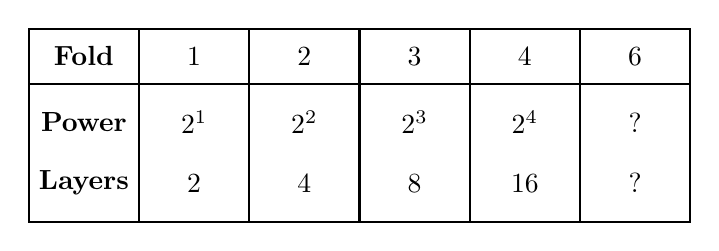
\begin{tikzpicture}[scale=0.7]
\draw[thick] (0,0) rectangle (12,3.5);
\draw[thick] (0,2.5) -- (12,2.5);
\draw[thick] (2,0) -- (2,3.5);
\draw[thick] (4,0) -- (4,3.5);
\draw[thick] (6,0) -- (6,3.5);
\draw[thick] (8,0) -- (8,3.5);
\draw[thick] (10,0) -- (10,3.5);
\node[font=\bfseries] at (1,3) {Fold};
\node at (3,3) {$1$};
\node at (5,3) {$2$};
\node at (7,3) {$3$};
\node at (9,3) {$4$};
\node at (11,3) {$6$};
\node[font=\bfseries] at (1,1.8) {Power};
\node at (3,1.8) {$2^1$};
\node at (5,1.8) {$2^2$};
\node at (7,1.8) {$2^3$};
\node at (9,1.8) {$2^4$};
\node at (11,1.8) {$?$};
\node[font=\bfseries] at (1,0.7) {Layers};
\node at (3,0.7) {$2$};
\node at (5,0.7) {$4$};
\node at (7,0.7) {$8$};
\node at (9,0.7) {$16$};
\node at (11,0.7) {$?$};
\end{tikzpicture}
\end{center}
\end{questionText}
\correctAnswer{$2^6 = 64$ layers}
\explanation{The pattern is $2^n$ layers after $n$ folds. After fold $6$: $2^6 = 64$ layers.}
\end{practiceQuestion}
